\documentclass{beamer}
\usepackage[utf8]{inputenc}
\usepackage{xeCJK} 
\usepackage[T1]{fontenc}
\usepackage{mathabx}
\usepackage{amsmath} 
\usepackage{mathpazo}
\usepackage{bibentry}

\usetheme{Boadilla}
\usecolortheme{wolverine}
\useoutertheme{miniframes}

\title{VP160 Recitation Class II}
\subtitle{Kinematics}
\author{Zeyi Ren}
\institute{UM-SJTU Joint Institute}

\begin{document}

\maketitle

\frame{\tableofcontents}

\section{Cartesian Coordinates}
\begin{frame}{Kinematics in 3D: Cartesian Coordinates}
  By convention, we write$$
  \frac{d\alpha}{dt}=\dot{\alpha},\quad \frac{d^2\alpha}{dt^2}=\ddot{\alpha}$$for convenience.\pause
  \begin{block}{Basic formulas in Cartesian Coordinates}
  $$ 
  \vec{r} = x\hat{n_x} + y\hat{n_y} + z\hat{n_z}$$
  $$
  \vec{v} = \dot{x}\hat{n_x} + \dot{y}\hat{n_y} + \dot{z}\hat{n_z}$$
  $$
  \vec{a} = \ddot{x}\hat{n_x} + \ddot{y}\hat{n_y} + \ddot{z}\hat{n_z}
  $$
\end{block}
\end{frame}

\section{Cylindrical and Spherical Coordinates}
\begin{frame}{Kinematics in 3D: Cylindrical Coordinates}
  \begin{block}{Basic Formulas in Cylindrical Coordinates}
    \begin{align*}\vec{r}&=\rho\hat{n_\rho}+z\hat{n_z}\\
  \vec{v}&=\dot{\rho}\hat{n_\rho}+\rho\dot{\phi}\hat{n_\phi}+\dot{z}\hat{n_z}\\
  \vec{a}&=(\ddot{\rho}-\rho\dot{\phi}^2)\hat{n_\rho}+(\rho\ddot{\phi}+2\dot{\rho}\dot{\phi})\hat{n_\phi}+\ddot{z}\hat{n_z}
  \end{align*}
  % $$\vec{r}=\rho\hat{n_\rho}+z\hat{n_z}$$
  %   $$\vec{v}=\dot{\rho}\hat{n_\rho}+\rho\dot{\phi}\hat{n_\phi}+\dot{z}\hat{n_z}$$
  %   $$\vec{a}=(\ddot{\rho}-\rho\dot{\phi}^2)\hat{n_\rho}+(\rho\ddot{\phi}+2\dot{\rho}\dot{\phi})\hat{n_\phi}+\ddot{z}\hat{n_z}
  %   $$
\end{block}\pause
  \textcolor{blue}{Tips:}\\
  \begin{itemize}
    \item if $z=0$, they become kinematics formulas in polar coordinates(see next slide).\pause
    \item Very useful, do remember this set of formulas, otherwise you may have to
    derive them by yourselves during the exam!
  \end{itemize}
\end{frame}

\section{Polar Coordinates}
\begin{frame}{Kinematics in 2D: Polar Coordinates}
  \begin{block}{Basic Formulas in Polar Coordinates}
    \begin{align}\vec{r}&=r\hat{n_r}\\
      \vec{v}&=\dot{r}\hat{n_r}+r\dot{\theta}\hat{n_\theta}\\
      \vec{a}&=(\ddot{r}-r\dot{\theta}^2)\hat{n_r}+(r\ddot{\theta}+2\dot{r}\dot{\theta})\hat{n_\theta}
      \end{align}
  Can be seen as a special case of cylindrical coordinates when $z=0$.
  \end{block}\pause
  \begin{block}{Relations with cartesian coordinates}
    $$x=rcos\theta,\ y=rsin\theta$$
    $$d\vec{r}=dr\hat{n_r}+rd\theta\hat{n_\theta},\ |d\vec{r}|=\sqrt{(dr)^2+(rd\theta)^2}$$
  \end{block}
\end{frame}

\begin{frame}
  \textcolor{blue}{Examples}
  \begin{figure}[htbp]
  \centering
  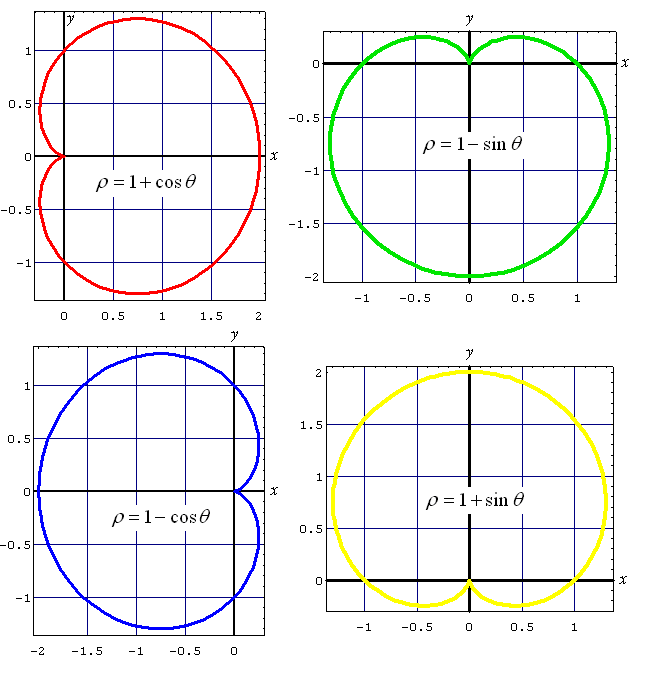
\includegraphics[width=0.5 \linewidth, angle =0]{CardioidsLabeled.png}
  \caption{Cardiod.}
  \label{fig:1}
  \end{figure}
\end{frame}

\begin{frame}
  \textcolor{blue}{Examples}
  Lemniscate:$$ r^2 = 2A^2 cos 2\theta.$$
  \begin{figure}[htbp]
    \centering
    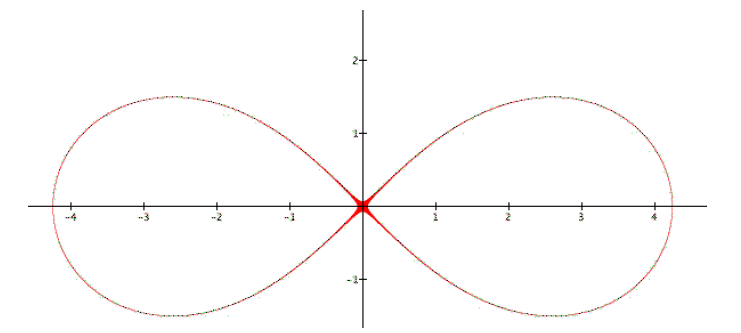
\includegraphics[width=0.8 \linewidth, angle =0]{Lemniscate.png}
    \caption{Lemniscate.}
    \label{fig:2}
    \end{figure}
\end{frame}

\begin{frame}
\textcolor{blue}{Exercise 1}

How to derive this set of formula$(1)(2)(3)$?\\ \pause
~\\
~\\
~\\
~\\
~\\
~\\
\textcolor{blue}{Tips:}\\
If you can derive it by yourself, you can be very confident about kinematics problems in exams.
\end{frame}

\section{Natural Coordinates}
\begin{frame}{Kinematics in 3D: Natural Coordinates}
  \begin{block}{Basic Vectors}
    \begin{enumerate}
      \item $\hat{n_\tau}:$ along the direction of $\vec{v}$
      \item $\hat{n_n}$ and $\hat{n_b}$: perpendicular to the direction of $\vec{v}$
    \end{enumerate}
    $$
      \hat{n_\tau}=\frac{\vec{v}}{|\vec{v}|},\ 
      \hat{n_n}=\frac{\dot{\hat{n_\tau}}}{|\dot{\hat{n_\tau}}|},\ 
      \hat{n_b}=\hat{n_\tau}\times \hat{n_n}
      $$
  \end{block}\pause
  \begin{block}{Basic Formulas}
    $$\vec{v}=v\hat{n_\tau}$$
    $$\vec{a}=\dot{v}\hat{n_\tau}+\frac{v^2}{R_c}\hat{n_n}$$
    $R_c$ means radius of curvature, what is radius of curvature?
  \end{block}
\end{frame}

\begin{frame}
  \textcolor{blue}{Important Tips}
  \begin{enumerate}
    \item Difference between $\dot{\vec{v}}$ and $\dot{v}.$\pause
    \item Difference between \textcolor{red}{normal and tangential}, \textcolor{brown}{radial and transversal} components of velocity and acceleration.
  \end{enumerate}
\end{frame}


\begin{frame}{Kinematics in 3D: Spherical Coordinates (Optional)}
  \begin{block}{Basic Formulas in Spherical Coordinates}
  \begin{align*}
    \vec{r}&= r\hat{n_r}\\
    \vec{v}&= \dot{r}\hat{n_r}+r cos\phi\dot{\theta}\hat{n_\theta}+r\dot{\phi}\hat{n_\phi}\\
    \vec{a}&= (\ddot{r}-r\dot{\theta}^2cos^2 \phi-r\dot{\phi}^2)\hat{n_r}\\ & +(2\dot{r}\dot{\theta}cos\phi-2r\dot{\theta}\dot{\phi}sin\phi+r\ddot{\theta}cos\phi)\hat{n_\theta}\\ & +(2\dot{r}\dot{\phi}+r\dot{\theta}^2cos\phi sin\phi+r\ddot{\phi})\hat{n_\phi}
    \end{align*}
  \end{block}\pause
  How to derive them?
  \textcolor{blue}{\url{http://output.to/sideway/default.aspx?qno=140700003}}
\end{frame}

\begin{frame}
\textcolor{blue}{Exercise 2}\\
\textcolor{blue}{\footnotesize{Cartesian coordinates and natural coordinates}}\\
A particle moves in the $x$-$y$ plane so that$$x(t) = at,\ y(t) = bt^2,$$
where $a, b$ are positive constants. Find its trajectory, velocity, and acceleration (its tangential and
normal components).
\end{frame}

\section{Exercises}
\begin{frame}
  \textcolor{blue}{Exercise 3}\\
  \textcolor{blue}{\footnotesize{Cartesian coordinates and natural coordinates}}\\
  The velocities of two particles observed from a fixed frame of reference are given in the Cartesian
  coordinates by vectors $\vec{v_1}(t) = (0, 2, 0) + (3, 1, 2)t^2$ and $\vec{v_2}(t) = (1, 0, 1).$ At the initial instant of
  time $t = 0$, the positions of these particles are $\vec{r_1}(0) = (1, 0, 0)$ and $\vec{r_2}(0) = (0, 1, 1).$
  \\
  ~\\ \textbf{Find}: the positions of both particles and the acceleration of particle 1 (and its tangential and normal
  components), relative position, and relative acceleration of particle 1 with respect to particle 2 at
  any instant of time $t$.
  \end{frame}

  \begin{frame}
  \textcolor{blue}{Exercise 4}\\
  \textcolor{blue}{\footnotesize{Polar coordinates (Archimedes' spiral)}}\\
  
  A disc of radius $R$ rotates about its axis of symmetry (perpendicular to the disk
surface) with constant angular velocity $\dot{\varphi}=\omega=$ const. At the instant of time $t = 0$ a beetle starts
to walk with constant speed $v_0$ along a radius of the disk, from its center to the edge.\\
\textbf{Find}\\
  (a) the position of the beetle and its trajectory in the Cartesian and polar coordinate systems,\\
  (b) its velocity both systems,\\
  (c) its acceleration in both systems (Cartesian components, polar components, as well as tangential
  and normal components).
\end{frame}

\begin{frame}
\textcolor{blue}{Exercise 5}\\
\textcolor{blue}{\footnotesize{Polar coordinates}}

A particle moves along a hyperbolic spiral (i.e. a curve $r=c/\varphi$, where $c$ is a positive constant), so
that $\varphi(t) = \varphi_0 + \omega t,$ where $\varphi_0$ and $\omega$ are positive constants. \textbf{Find} its velocity and acceleration (all
components and magnitudes of both vectors).
\end{frame}

\begin{frame}
\textcolor{blue}{Exercise 6}

For the situation discussed in \textcolor{blue}{Exercise 3},  answer the following questions.\\
(a) What is the distance covered by the beetle (write down the integral only, do not evaluate it)?\\
(b) What is the radius of curvature of the trajectory?
\end{frame}

\begin{frame}
\textcolor{blue}{Exercise 7}

Four spiders are initially placed at the four corners of a square with side length $a$. The spiders
crawl counter-clockwise at the same speed and each spider crawls directly toward the next spider
at all times. They approach the center of the square along spiral paths.\\ \textbf{Find}\\
(a) polar coordinates of a spider at any instant of time, assuming the origin is at the center of the
square,\\
(b) the time after which all spiders meet,\\
(c) the trajectory of a spider in polar coordinates.
\end{frame}

\begin{frame}
\textcolor{blue}{Exercise 8 (supplement)}

The hall chandelier with a height of $h$ above the ground exploded into fragments, shooting in all directions, the initial velocity was the same as $v_0$, and the fragments would not bounce when them reach the ground. Try to find the radius $R$ of the debris distribution area on the ground.
\begin{figure}[htbp]
\centering
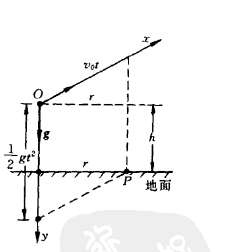
\includegraphics[width=0.4 \linewidth, angle =0]{ex8.png}
%\caption{.}
\label{fig:3}
\end{figure}
\end{frame}

\begin{frame}
\textcolor{blue}{Exercise 9 (supplement)}

Using kinematics method to solve the distribution function $\rho(x)$ of the radius of curvature of the curve $y=e^x$.
\begin{figure}[htbp]
\centering
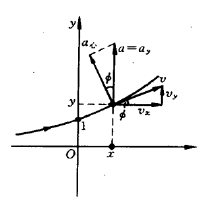
\includegraphics[width=0.45 \linewidth, angle =0]{ex9.png}
%\caption{.}
\label{fig:4}
\end{figure}
\end{frame}

\begin{frame}
\textcolor{blue}{Exercise 10 (supplement)}

The height of the river bank is $h$, and people use ropes to pull the boat to shore. If the angle between the rope and the water surface is $\theta$, the speed of the human left is $v_0$ and the acceleration is $a_0$. Try to find the speed $v$ and acceleration $a$ of the ship at this time.
\begin{figure}[htbp]
\centering
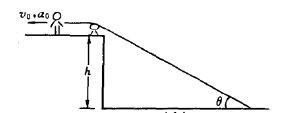
\includegraphics[width=0.5 \linewidth, angle =0]{ex10.png}
%\caption{.}
\label{fig:5}
\end{figure}
\end{frame}

% \section{Problems in HW1}
% \begin{frame}
% \textcolor{blue}{Problem 5} 

% Recall that $\textbf{r} = x\hat{n_x}+y\hat{n_y}+z\hat{n_z}$ is the position vector pointing from the origin $(0; 0; 0)$ to a
% point in space with the Cartesian coordinates $(x, y, z)$. Use what you know about vectors
% to show the following: All points $(x, y, z)$ that satisfy the equation $Ax + By + Cz = 0$,
% where $A$, $B$, and $C$ are constants, lie in a plane that passes through the origin and that
% is perpendicular to the vector $A\hat{n_x} + B\hat{n_y} + C\hat{n_z}$.
% \end{frame}

% \begin{frame}
% \textcolor{blue}{Problem 6(b)}

% Show that, for any $t$, the vectors $\textbf{n}$ and $\dot{\textbf{n}}$ are perpendicular to each
% other.
% \end{frame}





% \begin{frame}{Before We Start}
%   \begin{block}{What's in RC}
%     \begin{enumerate}
%       \item Basically two parts, conceptual part and exercises.
%       \item A brief review of concepts.
%       \item Exercises problems with hand-written notes, including some useful models that you may use in your assignments and exams.
%     \end{enumerate}
%   \end{block}
%   \pause
%   \begin{block}{What you can do}
%     \begin{enumerate}
%       \item Stop me and ask question directly at any time.
%       \item Basically anything but do not disturb your classmates.
%       \item Come to my OH just after RC, if you need one-to-one help.
%     \end{enumerate}
%   \end{block}
%   \pause
%   \textbf{The fewer fundamental principles you use to solve problems, the better your understanding of physics.}
% \end{frame}

% \section{Units}
% \begin{frame}
%   \begin{enumerate}[1.]
%     \item Scientific Notations
%     \begin{itemize}
%       \item $ a\times 10^n$ ($1\leq |a| < 10$)
%       \item Usually used for very large number or very small number like computation in Astrophysics or Quantum Mechanics.
%     \end{itemize}
%     \pause
%     \item Unit Prefix and Conversion
%     \begin{itemize}
%       \item \textcolor{red}{$k$} (unit prefix) \textcolor{blue}{$m$} (unit)
%       \item Some commonly-used unit prefixes:\\ 
%       \begin{table}[H]
%         \begin{tabular}{c|c|c|c|c|c|c|c}
%         \hline
%         $p$        & $n$       & $\mu$     & $m$       & $c$       & $k$      & $M$      & $G$      \\ \hline
%         $10^{-12}$ & $10^{-9}$ & $10^{-6}$ & $10^{-3}$ & $10^{-2}$ & $10^{3}$ & $10^{6}$ & $10^{9}$ \\ \hline
%         \end{tabular}
%         \end{table}
%         \pause
%         CASIO fx-991CN X $\rhd$ $\boxed{OPTN}$ $\rhd$ $3:$工程符号\\
%         e.g.\\Input: 1m; Output: $\frac{1}{1000}$
%     \end{itemize}
%     \pause
%     \item Basic Units \& Derived Units
%     \begin{itemize}
%       \item SI system of units: 
%       \begin{table}[H]
%         \begin{tabular}{c|c|c|c|c|c|c|c}
%         \hline
%         Quantity & $L$        & $m$       & $t$       & $I$       & $T$       & $n$      & $lv$     \\ \hline
%         Unit     & \textcolor{black}{$m$} & $kg$& $s$ & $A$ & $K$ & $mol$ & $cd$ \\ \hline
%         \end{tabular}
%         \end{table}
%     \end{itemize}
%   \end{enumerate}
% \end{frame}

% \begin{frame}{Dimensional Analysis: System of Units}
% \begin{enumerate}
%   \item We can first select some physical quantities as the ``\textbf{basic quantities}”
%   and specify a ``\textbf{unit for measurement}” for each basic quantity,
%   the other physical quantities' units can be derived from the
%   relation between them and the fundamental
%   quantities. These physical quantities are called \textbf{derived quantities}
%   and their units It's called \textbf{derived unit}.
%   \pause
%   \item A set of units derived in this way, is called a \textbf{system of units}.
%   \pause
%   \item We often use capital letter to represent a ``dimensional quantity", and
%   use [$x$] to represent the ``dimensional quantity" of specific physical quantity $x$.\\
%   \pause
%   e.g. The dimensional quantity of a particle of mass $m$ is written as: $M$ = [$m$].
% \end{enumerate}
% % \end{block}
% \end{frame}

% \begin{frame}
%   \textcolor{blue}{Exercise 1}\\
%   A simple pendulum consists of a light inextensible string AB with length $l$, with the end $A$ fixed, and a point mass $m$ attached to $B$. The pendulum oscillates with a small amplitude, and the period of oscillation is $T$. It is suggested that $T$ is proportional to the product of powers of $m$, $l$ and $g$, where $g$ is the acceleration due to gravity. Use dimensional analysis to find this relationship. 
% \end{frame}

% \section{Uncertainty and Significant Figures}
% \begin{frame}{Uncertainty}
%   \begin{enumerate}
%     \item Because of limitations of measurement devices, imperfect
%     measurement procedures and randomness of environmental
%     conditions, as well as human factors related to the experimenter
%     himself, no measurement can ever be perfect. Its result may therefore
%     only be treated as an estimate of what we call the ``exact value” of a
%     physical quantity. The experiment may both overestimate and
%     underestimate the value of the physical quantity, and it is crucial to
%     provide a measure of the error, or better uncertainty, that a result of
%     the experiment carries (cited from ``Introduction to Measurement
%     Data Analysis” in VP141).
%     \pause
%     \item The detailed calculation will be encountered in VP141. The principles of uncertainty analysis will be explained in VE401.
%   \end{enumerate}
% \end{frame}

% \begin{frame}{Significant Figures} 
%     \begin{enumerate}
%       \item Experimental uncertainty should almost always be rounded to one significant figure. The only exception is when the uncertainty has a leading digit of 1, then we can keep two significant figures (you may encounter this in VP141).
%       \pause
%       \item The significant figure required in VP160 is not so strict.
%     \end{enumerate}
%     \pause 
%     \textcolor{blue}{Example}
%     \begin{enumerate}
%       \item $1.7392$ ($SF = 5$)
%       \item $0.0970$ ($SF = 3$)
%       \item $3.7\times 10^5$ ($SF = 2$)
%       \item $5.00\times 10^3$ ($SF = 3$)
%     \end{enumerate}
%   % \end{block}
% \end{frame}

% \section{Fermi Problems}
% \begin{frame}{Back-of-the-envelop Problems}
%   \begin{block}{Definition}
%     A quick estimation of some physical quantities. Also called ``Fermi problems''. Named after the American physicist Enrico Fermi.
%   \end{block}
%   \pause
%   \begin{block}{Tips}
%     \begin{enumerate}
%       \item Try to remember the order of magnitude of some important constant.
%       \item This type of questions may occur in exams.
%     \end{enumerate}
%   \end{block}
%   \pause
%   \textcolor{blue}{Exercise 2.1}\\
%   True or False: The power of China Railway High-speed (CRH) is about 500kW.\\
%   (False)\\
% \end{frame}

% \begin{frame}
%   \textcolor{blue}{Exercise 2.2} (just for fun)\\
%   Fermi's estimation of nuclear explosion: Fermi held a scrap of paper at the height of his head and released while at the same time, an atomic bomb exploded in New Mexico, the scrap of paper fell on the floor with a horizontal displacement of $2.5m$. How many tons of TNT this explosion is equivalent to?
% \end{frame}

% \section{Vectors}
% \begin{frame}
%   \begin{block}{Difinition}
%     Vectors are quantities that have both \textcolor{red}{magnitude} and \textcolor{red}{direction}.
%   \end{block}
%   \pause
%   \begin{table}[]
%     \begin{tabular}{c|c}
%     \hline
%     \textbf {Scalar}                                                      & \textbf {Vector}                                                             \\ \hline
%     \begin{tabular}[c]{@{}c@{}}Distance\\ Speed\end{tabular} & \begin{tabular}[c]{@{}c@{}}Displacement\\ Velocity\end{tabular} \\ \hline
%     \end{tabular}
%     \end{table}
%     \pause
%     \begin{block}{Vectors in $\mathbb{R} ^n$}
%       $\vec{u} = $ ($u_1,u_2,...,u_n $)$^T$
%     \end{block}
% \end{frame}

% \begin{frame}{Basic Vector operations}
%   \begin{itemize}
%     \item Addition \& Subtraction\\ $$\vec{u}\pm \vec{v}=(u_1\pm v_1,u_2\pm v2,u_3\pm v_3)$$ 
%     \item Scalar Multiplication$$\lambda \vec{u} = (\lambda u_1, \lambda u_2, \lambda u_3)$$
%     \item Dot Product$$\vec{u}\cdot \vec{v} = |u||v|cos\theta=u_1v_1+u_2v_2+u_3v_3$$
%     \item Orthogonal Projection Vector of the vector $\vec{u}$ onto the vector $\vec{v}$$$\frac{\vec{u}\cdot \vec{v}}{|\vec{v}|}\cdot \frac{\vec{v}}{|\vec{v}|}$$
%   \end{itemize}
% \end{frame}

% \begin{frame}{Basic Vector operations}
%   \begin{itemize}
%     \item Cross Product
%     \begin{itemize}
%       \item Magnitude: $|\vec{u}\times \vec{v}|=|\vec{u}||\vec{v}|sin\theta$
%       \item Direction: determined by \textbf{Right Hand Rule}
%       \item Matrix expression(Using determinant):
%       \begin{align*}
%         \vec{u}\times \vec{v} &= \left|\begin{matrix}\hat{i}&\hat{j}&\hat{k}\\u_1 & u_2 & u_3\\ v_1 & v_2 & v_3 \end{matrix}\right|\\&=(u_2v_3-u_3v_2)\hat{i}+(u_3v_1-u_1v_3)\hat{j}+ (u_1v_2-u_2v_1)\hat{k}
%  \end{align*}
%     \end{itemize}\pause
%     \item Triple Product
%     \begin{itemize}
%       \item Scalar Triple Product:$$\vec{u}\cdot(\vec{v}\times \vec{w})=\vec{v}\cdot(\vec{w}\times \vec{u})=\vec{w}\cdot(\vec{u}\times \vec{v})$$
%       \item Vector Triple Product:$$\vec{u}\times (\vec{v}\times \vec{w})=\vec{v}(\vec{u}\cdot\vec{w})-\vec{w}(\vec{u}\cdot \vec{v})$$
%     \end{itemize}
%   \end{itemize}
% \end{frame}

% \begin{frame}
% \textcolor{blue}{Exercise 3.1}

% Consider two vectors $ \vec{u}= 3\hat{n_x} +4\hat{n_y}$, and $\vec{w}= 6\hat{n_x} +16\hat{n_y}$. Find:\\
% (a) the components of the vector $\vec w$ that are parallel and perpendicular
% to the vector $\vec u$,\\
% (b) the angle between $\vec w$ and $\vec u$.
% \end{frame}

% \begin{frame}
% \textcolor{blue}{Exercise 3.2}

% Check that in Cartesian coordinates, the two expression equations
% of dot product of two vectors $\vec{u}$ and $\vec{v}$ are equivalent:$$\vec{u}\cdot \vec{v} = u_1v_1 + u_2v_2 + u_3v_3$$
% $$\vec{u}\cdot \vec{v} = |\vec{u}||\vec{v}|cos\theta$$
% \end{frame}

% \begin{frame}
% \textcolor{blue}{Exercise 3.3}

% Prove:$$
% \vec{u}\times (\vec{v}\times \vec{w})+\vec{v}\times(\vec{w}\times \vec{u})+\vec{w}\times(\vec{u}\times\vec{v})=0$$
% Then check \textbf{under what circumstance} the associativity of vector triple product stands, that is $$\vec{u}\times (\vec{v}\times \vec{w}) = (\vec{u}\times \vec{v})\times \vec{w}$$
% (In general, this equation does not hold)
% \end{frame}

% \section{3D Curvilinear Coordinate system}
% \begin{frame}{Cartesian Coordinate}
%   \begin{enumerate}
%     \item Coordinates: $x, y, z$
%     \item Unit Vectors: $\hat{n_x}, \hat{n_y}, \hat{n_z}$
%     \item Position Vector: $\vec{r} = x\hat{n_x}+y\hat{n_y}+z\hat{n_z}$
%   \end{enumerate}
% \end{frame}

% \begin{frame}{Cylindrical Coordinate}
%   \begin{enumerate}
%     \item Coordinates: $\rho, \phi, z$
%     \item Unit Vectors: $\hat{n_\rho}, \hat{n_\phi}, \hat{n_z}$
%     \item Position Vectors: $\vec{r} = \rho\hat{n_\rho}+z\hat{n_z}$
%     \item Relationship with Cartesian Coordinates:
%     $$\left\{\begin{array} { l } 
%       { \rho = \sqrt { x ^ { 2 } + y ^ { 2 } } } \\
%       { \phi = \operatorname { a r c t a n } ( y / x ) } \\
%       { z = z }
%       \end{array} \quad \left\{\begin{array}{l}
%       x=\rho \cos (\theta) \\
%       y=\rho \sin (\phi) \\
%       z=z
%       \end{array}\right.\right.$$
%   \end{enumerate}
% \end{frame}

% \begin{frame}{Spherical Coordinate}
%   \begin{enumerate}
%     \item Coordinates: $r, \phi, \theta$
%     \item Unit Vectors: $\hat{n_r}, \hat{n_\phi}, \hat{n_{\theta}}$
%     \item Position Vector: $\vec{r} = r\hat{n_r}$
%     \item Relationship with Cartesian Coordinate:$$\left\{\begin{array} { l } 
%       { r = \sqrt { x ^ { 2 } + y ^ { 2 } + z ^ { 2 } } } \\
%       { \phi = \operatorname { a r c t a n } ( y / x ) } \\
%       { \theta = \operatorname { a r c t a n } ( \sqrt { x ^ { 2 } + y ^ { 2 } } / z ) }
%       \end{array} \quad \left\{\begin{array}{l}
%       x=\rho \sin (\theta) \cos (\phi) \\
%       y=r \sin (\theta) \sin (\phi) \\
%       z=r \cos (\theta)
%       \end{array}\right.\right.$$
%   \end{enumerate}
% \end{frame}

% \begin{frame}
% \textcolor{blue}{Exercise 4.1}

% Derive the above relation equations.
% \end{frame}

% \begin{frame}
% \textcolor{blue}{Exercise 4.2}

% Using Spherical Coordinate, calculate the volume of the solid-line part showed below
% \begin{figure}[htbp]
% \centering
% 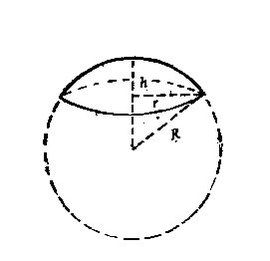
\includegraphics[width=0.5 \linewidth, angle =0]{qiuque.png}
% % \caption{Exercise 5.2}
% % \label{fig:1}
% \end{figure}
% \end{frame}

% \section{1D Kinematics}
% \begin{frame}
%   \begin{itemize}
%     \item Average vs. Instantaneous Quantities$$v_{x,A} = \frac{x(t+\Delta t)-x(t)}{\Delta t}\quad a_{x,A} = \frac{v(t+\Delta t)-v(t)}{\Delta t}$$
%     \item Relationships\begin{align*}
%     x &= x(t)\\
%     v &= v(t)=\frac{d}{dt} x(t)\\
%     a &= a(t)=\frac{d}{dt} v(t)=\frac{d^2}{dt^2}x(t)  
%     \end{align*}
%     \item Relative motion$$x = x_r + x';\quad v = v_r+v';\quad a=a_r+a'$$
%   \end{itemize}
% \end{frame}

% \begin{frame}
% \textcolor{blue}{Exercise 5.1}

% A car is moving in one direction along a straight line. Find the average velocity of the car if:\\
% (a) it travels half of the journey time with velocity $v_1$ and the other
% half with velocity $v_2$,\\
% (b) it covers half of the distance with velocity $v_1$ and the other
% one with velocity $v_2$.
% \end{frame}

% \begin{frame}
% \textcolor{blue}{Exercise 5.2}

% A particle is moving along a straight line with velocity $v_x(t) =
% -\beta A\omega e^{-\beta}cos\omega t$, where $A, \omega$, and $\beta$ are positive constants. Assuming
% that $x(0) = 5m$.\\
% (a) What are the units of these constants?\\
% (b) Find acceleration $a_x (t)$ and position $x(t)$ of the particle.\\
% (c) Sketch the graphs of $x(t)$, $v_x (t)$, and $a_x (t)$.\\
% (d) What kind of motion may these results describe?
% \end{frame}

% \begin{frame}
% \textcolor{blue}{Exercise 5.3}

% In a certain motion of a particle along a straight line, the acceleration
% turns out to be related to the position of the particle according to the formula $a_x = \sqrt{kx}$, where $k > 0$ is a constant
% and $x > 0$. How does the velocity depend on x, if we know that
% for $v_x (x_0) = v_0$?
% \end{frame}

% \begin{frame}
% \textcolor{blue}{Exercise 5.4}

% A dripping water faucet steadily releases drops $1$drop/s apart. As
% these drops fall, does the distance between them decrease, increase,
% or remain the same? (Try to find the answer without calculation)
% \end{frame}

% \begin{frame}
% \textcolor{blue}{Exercise 5.5}

% A spare paddle drops from a fisherman’s canoe. After one hour
% of paddling the fisherman realizes that the paddle is missing.
% He turn around and paddles his canoe back to find the paddle.
% Assume that the fisherman paddles always with the same speed
% $v = 10km/h$ with respect to the river, the speed of the rivers
% current is $u = 6km/h$. Find:\\
% (a) the time that the fisherman takes to find the paddle;\\
% (b) the distance between the places where the paddle drops and
% the fisherman find it.\\
% Can you find the answers within a second?
% \end{frame}

\begin{frame}{Reference}
  \begin{thebibliography}{9}
  \setbeamertemplate{bibliography item}[article]
  \bibitem{C} Yigao Fang.\\
  \textcolor{black}{VP160 Recitation Slides.}\\
  2020
  \bibitem{C} Haoyang Zhang.\\
  \textcolor{black}{VP160 Recitation Slides.}\\
  2020
  \setbeamertemplate{bibliography item}[book]
  \bibitem{C} Yousheng Shu (舒幼生).\\
  \textcolor{black}{\textit{Mechanics (力学)}}\\
  Peking University Press, 2005
  \end{thebibliography}
  \end{frame}

  \end{document}



